%%===============================================================================
% Document configuration

%%-------------------------------------------------------------------------------
% Document type

%\documentclass[conference]{IEEEtran}
\documentclass[letterpaper, 10pt, conference]{IEEEtran}
% \IEEEoverridecommandlockouts

%%-------------------------------------------------------------------------------
% Package configuration
\usepackage{algorithmic}
\usepackage{amsmath,amsfonts}
\usepackage{booktabs, tabularx}   % allows for \toprule in tables
\usepackage{caption}
\usepackage{cite}
\usepackage{graphicx}
\graphicspath{ {./img/} }
\usepackage{multirow}
\usepackage{newtxmath}
\usepackage{pgfplots}
\usepackage{ragged2e}
\usepackage{subcaption}
\usepackage{textcomp}
\usepackage{tikz}
\usepackage{xcolor}

\usetikzlibrary{arrows.meta}

%%-------------------------------------------------------------------------------
% Custom Commands
\newcommand{\TODO}[1]{{\color{green} To do: #1}} % For adding notes to paper

%%-------------------------------------------------------------------------------
% Bibliography
\def\BibTeX{{\rm B\kern-.05em{\sc i\kern-.025em b}\kern-.08em
    T\kern-.1667em\lower.7ex\hbox{E}\kern-.125emX}}

%%-------------------------------------------------------------------------------
% Title
\title{A Position Allocation Approach to the Scheduling of Battery Electric Bus Charging}

%%-------------------------------------------------------------------------------
% Authors
\author{\IEEEauthorblockN{1\textsuperscript{st} Alexander Brown}
\IEEEauthorblockA{\textit{Department of Electrical and Computer Engineering} \\
\textit{Utah State University}\\
Logan, USA \\
alex.brown7711@aggiemail.usu.edu}
\and
\IEEEauthorblockN{2\textsuperscript{nd} Greg Droge}
\IEEEauthorblockA{\textit{Department of Electrical and Computer Engineering} \\
\textit{Utah State University}\\
Logan, USA \\
greg.droge@usu.edu }}

%%===============================================================================
% Title, Authors, Abstract, Keywords
\begin{document}

%%-------------------------------------------------------------------------------
% Create title
\maketitle

%%-------------------------------------------------------------------------------
% Abstract
\begin{abstract}
[\TODO{Copied}] A major challenge to adopting battery electric buses into bus fleets is the scheduling of the battery charging while considering route timing constraints, battery charge, and battery health. This work develops a scheduling framework to balance the use of slow and fast chargers assuming the bus routes and charger locations are fixed. Slow chargers are utilized when possible for sake of battery health and fast chargers are used when needed to accommodate timing constraints and ensure a sufficient charge for route execution. A directed, acyclic graph is used to model the available charge times for buses that periodically return to a depot for charging. A constrained network flow Mixed-Integer Linear Program (MILP) problem is formulated to optimize the scheduling of chargers as well as to determine the number of chargers required to meet charging thresholds. Results are presented using a randomly generated bus schedule for thirty buses and demonstrate the ability of the planner to consider peak time charging costs while planning with fixed and variable numbers of chargers.
\end{abstract}

%%-------------------------------------------------------------------------------
% Keywords
\begin{IEEEkeywords}

\end{IEEEkeywords}

%%===============================================================================
% Paper

%%-------------------------------------------------------------------------------
% Introduction
\section{Introduction}
\label{sec:introduction}
The public transportation system is crucial in any urban area; however, the increase awareness and concern of environmental impacts of petroleum based public transportation has driven an effort to reduce the pollutant footprint \cite{DeFilippo2014, Xylia2018, Guida2017, Li2016}. Particularly, the electrification of public bus transportation via battery power, i.e., battery electric buses (BEBs), has received significant attention \cite{Li2016}. Although the technology provides benefits beyond reduction in emissions such as lower driving costs, lower maintenance costs, and reduced vehicle noise, battery powered systems introduce new challenges such as larger upfront costs, and potentially several hour long ``refueling" periods \cite{Xylia2018, Li2016}. Furthermore, the problem is exacerbated by the constraints of the transit schedule the fleet must adhere to, the limited amount of chargers available, as well as the adverse affects in the health of the battery due to fast charging \cite{Lutsey2019}. This paper presents a continuous scheduling framework for a BEB fleet that shares limited fast and slow chargers. This framework takes into consideration linear charging dynamics and a fixed bus schedule while meeting a certain battery percentage threshold while remaining.

[\TODO{Copied}] Recent research seeks to enable BEB fleet deployment by solving two problems: providing BEB scheduling (when to charge, at which charger) and determining BEB infrastructure (charger placement, route design). Much attention has been given to solving both problems simultaneously \cite{Wei2018, Sebastiani2016, Hoke2014, Wang2017}. Additional variations in addressing the infrastructure include determining which existing buses should be replaced by a BEB \cite{Zhou2020}, assignments of buses to routes \cite{Liu2020}, and determining locations of fast wireless chargers along the routes \cite{Yang2018, Wang2017a}. The added complexity of considering both the BEB charge scheduling and the infrastructure problems necessitates simplifications for sake of computation.

[\TODO{Copied}] Two such simplifications are common. First, only fast chargers are utilized in planning \cite{Wei2018, Sebastiani2016, Wang2017, Zhou2020, Liu2020, Yang2018, Wang2017a, Qin2016}. Second, significant simplifications to the charging models are made. Some approaches assume full charge \cite{Wei2018, Wang2017, Zhou2020, Wang2017a}. Others have assumed that the charge received is proportional to the time spent on the charger \cite{Liu2020, Yang2018}, which can be a valid assumption when the battery state-of-charge (SOC) is below 80\% charge \cite{Liu2020}. Day-to-day operations require higher fidelity charging models to ensure buses have sufficient charge and to better incorporate the monetary cost of charging. In \cite{Sebastiani2016, Qin2016}, high-fidelity models are used at the price of requiring computationally intensive searches; \cite{Sebastiani2016} uses a genetic algorithm and \cite{Qin2016} uses an exhaustive search strategy.

The contribution of this work is a Mixed Integer Linear Program (MILP) scheduling framework that considers bus schedules, charging battery dynamics, charge limits, and availability of slow and fast chargers. The bus schedules are assumed to be fixed for the duration of the time horizon. The linear program is formed, and extends upon, the Position Allocation Problem (PAP) \cite{Qarebagh2019}. Linear charging dynamics are assumed, costs are assumed to be constant for the duration of the time horizon, and the amount of chargers is assumed to be constant. The MILP framework allows the addition and replacing of constraints. As such, battery dynamic constraints may be replaced with first-order dynamic modeling and costs can be made dynamic. The solution of the problem provides the arrival time, selected charger (fast or slow), initial charge time, final charge time, and departure time from the station.

The remainder of the paper proceeds as follows. \TODO{List out sections}

\begin{table*}[!t]
	\caption{Notation used throughout the paper}
	\label{tab:variables}
	\centering
	\begin{tabular}{l l l l}
		\toprule
		\textbf{Variable} & \textbf{Description} & \textbf{Variable} & \textbf{Description} \\
		\toprule
		\multicolumn{4}{l}{Input values} \\
			$A$           & Number of buses in use &
			$I$           & Final index                               \\
			$M$           & An arbitrary very large upper bound value &
			$N$           & Number of total visits                    \\
			$O$           & Bounding box for rectangle packing        &
			$\vmathbb{O}$ & Set of rectangles to be packed in \(O\)   \\
			$Q$           & Number of chargers                        &
			$T$           & Time Horizon                              \\
			$\Xi$         & $N(N-1)$                                  \\
		\hline
		\multicolumn{4}{l}{Input variables} \\
			$\Gamma_i$   & Array of visit id's                                             \\
			$\alpha_i$   & Initial charge time for visit  $i$                              &
			$\beta_{i}$  & Final charge for bus $i$ at the end of the work day             \\
			$\epsilon_q$ & Cost of using charger $q$ per unit time                         &
			$\gamma_i$   & Array of values indicating the next index visit $i$ will arrive \\
			$\kappa_i$   & Battery capacity for bus \(i\)                                  &
			$\lambda_i$  & Discharge of visit over route  $i$                              \\
			$\nu$        & Minimum charge allowed on depatrue of visit \(i\)               &
			$\tau_i$     & Time visit $i$ must leave the station                           \\
			$\upsilon$   & Minimum final percentage charge at and of time horizon \(T\)    &
			$a_i$        & Arrival time of visit  $i$                                      \\
			$m_q$        & Cost of a visit being assigned to charger  $q$                  &
			$r_q$        & Charge rate of charger $q$ per unit time                        \\
		\hline
		\multicolumn{4}{l}{Decision Variables} \\
			$\delta_{ij}$ & $v_i < v_j = 1$ \textrm{ or } $i \neq j = 0$                    &
			$\eta_i$      & Initial charge for visit $i$                                    \\
			$\sigma_{ij}$ & $u_i < u_j = 1$ \textrm{ or } $i \neq j = 0$                    &
			$c_i$         & detach time from charger for visit $i$                          \\
			$g_i$         & Linearization term for bilinear terms $g_i := p_i w_{iq}$       &
			$p_i$         & Amount of time spent on charger for visit $i$                   \\
			$u_i$         & Initial charge time of visit $i$                                &
			$v_i$         & Assigned queue for visit $i$                                    \\
			$w_{iq}$      & Vector representation of queue assignment                       \\
			\bottomrule
	\end{tabular}
\end{table*}

%%-------------------------------------------------------------------------------
% Preliminaries
\section{Preliminaries}
\label{sec:preliminaries}
The BEB charge schedule formulation in this work builds upon the PAP. The PAP is a rectangle packing problem where a set of rectangles \(\vmathbb{O}\) are attempted to be optimally placed in a larger rectangle \(O\) as shown in Fig \ref{fig:packexample}. Both the set \(\vmathbb{O}\) and rectangle \(O\)'s width and height are used to represent quantifiable values. The rectangle packing problem is a NP-hard problem that is a subset of the packing problem and can be used to describe many real life problems \cite{Bruin2013,Murata1995}. In some of these problems, the dimensions of \(\vmathbb{O}\) are held constant such as in the problem of packing modules on a chip, where the widths and height of the rectangles represent the physical width and heights of the modules \cite{Murata1995}. Other problems, such as the Berth Allocation Problem (BAP), allow one or both sides to be decision variables \cite{Buhrkal2010}.

The BAP is a form of the rectangle packing problem where the set of rectangles describe incoming vessels to a be docked on a berth to be serviced as shown in Fig \ref{fig:bapexample} \cite{Dai2008}. The BAP is commonly formed as a Mixed Integer Linear Program (MILP) \cite{Frojan2015,Buhrkal2010}. This formulation utilizes the BAP to help determine which queue the bus should be placed on to be charged without violating time or space constraints. Notation is summarized in Table \ref{tab:variables}.

\begin{figure}
	\centerline{\begin{tikzpicture}[scale=0.6]
        \draw [thick,<->] (0,7) node[above]{$Y$}--(0,0)--(7,0) node[right]{$X$};
	    \draw [thick, -] (0,0) rectangle (5,5) node[right]{$O$};
	    \draw (0,0) rectangle (5,5) node[right]{$O$};
	    \draw (0,0) rectangle (5,5) node[right]{$O$};
	\end{tikzpicture}}
	\caption{Example of rectangle packing problem \TODO{Update Image}}
	\label{fig:packexample}
\end{figure}

\begin{figure}
	\centerline{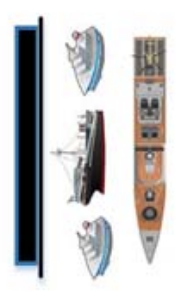
\includegraphics[height=4cm]{bapexample.png}}
	\caption{Example of berth allocation. Vessels flow from top to bottom.\TODO{Update Image}}
	\label{fig:bapexample}
\end{figure}

\subsection{The Berth Allocation Problem}
The BAP solves the problem of optimally assigning incoming vessels to berth positions to be serviced (Fig \ref{fig:bapexample}). The width and height of \(O\) represent the berth length \(S\) and time horizon \(T\), respectively. Similarly, the width and height for \(\vmathbb{O}\) represent the time spent to service vessel $i$ and the space taken by docking vessel $i$, respectively. The vessel characteristics (length of the vessel, arrival time, handling time, desired departure time) are assumed to be known for all $N$ vessels to be serviced. A representation of a BAP solution is shown in Fig \ref{fig:bap}.

The BAP objective is generally represented as minimizing some operational time for a given vessel \(i\). The operational time may be chosen to minimize time of arrival to time of departure, time spent being serviced, or overall waiting time (i.e. \(a_i \leq u_i\)) \cite{Cheng2007, Buhrkal2010,Frojan2015}. The model must then constrain the vessel placement as to not allow overlap in time or space as well as disallowing discontinuities in arrival times to departure times. The followng MILP describes the stated objective and constraints. The MILP is also shown in its entirety as it forms the foundation from which the PAP is constructed \cite{Qarebagh2019}.

\begin{figure}
	\centerline{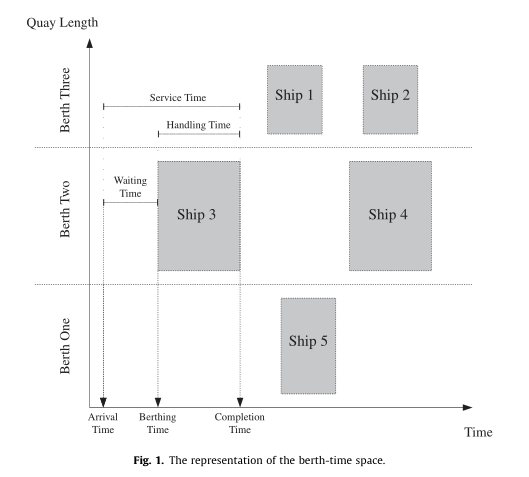
\includegraphics[width=8cm]{bap.png}}
	\caption{The representation of the berth-time space \TODO{Update Image}}
	\label{fig:bap}
\end{figure}

\begin{equation}
	\label{eq:bapobjective}
	min\; \sum_{i=1}^N (c_i - a_i)
\end{equation}

Subject to the following constraints:

\begin{subequations}
\label{eq:bapconstrs}
\begin{align}
    u_j - u_i - p_i - (\sigma_{ij} - 1)T \geq 0                     \label{subeq:baptime}         \\
    v_j - v_i - s_i - (\delta_{ij} - 1)S \geq 0                     \label{subeq:bapspace}        \\
    \sigma_{ij} + \sigma_{ji} + \delta_{ij} + \delta_{ji} \geq 1    \label{subeq:bapvalid_pos}    \\
    \sigma_{ij} + \sigma_{ji} \leq 1                                \label{subeq:bapsigma}        \\
    \delta_{ij} + \delta_{ji} \leq 1                                \label{subeq:bapdelta}        \\
    p_i + u_i = c_i                                                 \label{subeq:bapdetach}       \\
    a_i \leq u_i \leq (T - p_i)                                     \label{subeq:bapvalid_starts} \\
    \sigma_{ij} \in \{0,1\},\;\delta_{ij} \in \{0,1\}               \label{subeq:sdspace}
\end{align}
\end{subequations}

\noindent
Where for this problem the following are constants

\begin{itemize}
	\item \(S\)   : berth length
	\item \(T\)   : time horizon
	\item \(N\)   : number of incoming vessels
	\item \(p_i\) : charging time for vessel \(i\;; \forall 1 \leq i \leq N\)
	\item \(s_i\) : size of vehicle \(i\;; \forall 1 \leq i \leq N\)
	\item \(a_i\) : arrival time of vessel \(i\;; \forall 1 \leq i \leq N\)
\end{itemize}

\noindent
and the following are decision variables

\begin{itemize}
    \item \(u_i\)         : starting time of service for vessel \(i\;; \forall 1 \leq i \leq N\)
    \item \(v_i\)         : berth position \(i\;; \forall 1 \leq i \leq N\)
    \item \(c_i\)         : departure time for vessel \(i\;; \forall 1 \leq i \leq N\)
    \item \(\sigma_{ij}\) : \(u_i < u_j\;; \forall 1 \leq i < j \leq N\)
    \item \(\delta_{ij}\) : \(v_i < u_j\;; \forall 1 \leq i < j \leq N\)
\end{itemize}

The objective function \eqref{eq:bapobjective} minimizes the time spent to service each vessel by minimizing over the difference between the departure time (\(c\)) and arrival time (\(a\)).

Constraints \ref{subeq:baptime}-\ref{subeq:bapdelta} are the "queuing constraints". They are used to prevent overlapping over both space and time as shown in Fig \ref{fig:overlap}. In terms of the BAP, constraint \eqref{subeq:baptime} states that the starting service time (\(u\)) for vessel \(j\) must be greater than the starting time of vessel \(i\) plus its service time (\(p\)). The last term utilizes the Big-M notation to activate or deactivate the constraint. Specifically, \eqref{subeq:baptime} is active if both \(i\) and \(j\) are visiting the same berth (\(u_i = u_j\)). A value of \(\sigma_{ij} = 1\) will activate the constraint to ensure that \(i\) is complete before \(j\) is allowed to begin being serviced. If \(\sigma = 0\), then the constraint is of the form \(T + u_j + p_j > u_i\) rendering the constraint ``inactive" because \(u_i\) cannot be larger than \(T + u_j + p_j\).

In a similar fashion, \(\delta_{ij}\) effectively determines whether the vessel will be located in adjacent berths. If \(\delta_{ij} = 1\) then \eqref{subeq:bapspace} is rendered active and vessels \(i\) and \(j\) must be in adjacent berthing locations.

%Constraint \ref{subeq:bapspace} states that the berth location for vessel \(i\) is greater than the starting berth position of vessel \(j\) plus its length (no overlap in physical space on the berth) as shown in Fig \ref{subfig:spaceoverlap}. Again, the big \(M\) method is utilized to determine the relevance of the constraint. If \(\delta_{ij} = 1\) then the big \(M\) term goes to zero rendering the constraint active. If \(\delta_{ij} = 0\) then the constraint is inactive.

\begin{figure}
    \centering
    \begin{subfigure}[b]{0.2\textwidth}
        \centering
    	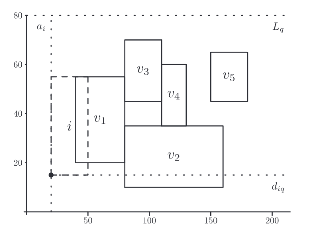
\includegraphics[height=3cm]{hoizontaloverlap.png}
    	\caption{Example horizontal overlap in time in time-space plot\TODO{Update Image}}
    	\label{subfig:timeoverlap}
	\end{subfigure}
	\hfill
    \begin{subfigure}[b]{0.2\textwidth}
        \centering
    	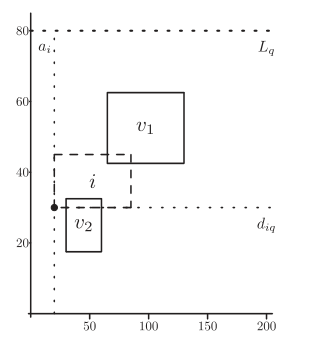
\includegraphics[height=3cm]{verticaloverlap.png}
    	\caption{Example of overlap in space in time-space plot\TODO{Update Image}}
    	\label{subfig:spaceoverlap}
	\end{subfigure}
	\caption{Visualization of vessel relative positions}
	\label{fig:overlap}
\end{figure}

Constraints \ref{subeq:bapvalid_pos}-\ref{subeq:bapdelta} are used to establish queuing by providing a relationship between queuing variables (\(u\) and \(v\)). Constraint \eqref{subeq:bapdelta} states that one of the following is true: \(u_i < u_j \iff \sigma_{ij} = 1\) or \(u_j < u_i \iff \sigma_{ji} = 1\), and \(v_i < v_j \iff \delta_{ij} = 1\) or \(v_j < v_i \iff \delta_{ji} = 1\). Constraints \eqref{subeq:bapsigma} and \eqref{subeq:bapdelta} enforce consistency, i.e. \(u_i < u_j\) and \(u_j < u_i\) cannot be simultaneously true. This enforces a relationship between vessels: either one is before the other temporally or they are in different queues.

%A useful way of describing \(\sigma_{ij}\) and \(\delta_{ij}\) are in terms of relative position of vessels on the time-space diagram. \(\delta_{ij} = 1\) implies \(i\) is ``to the left of" \(j\) and \(\sigma_{ij} = 1\) implies \(i\) ``is below" \(j\). If vessel \(i\) is to the left of \(j\) then \(i\) cannot intersect \(j\) vertically (\(\sigma_{ij} = 1\) and \(\delta_{ij} = 0\)), see Fig \ref{subfig:timeoverlap}. Similarly, if \(i\) is below \(j\) then \(i\) is unable to overlap \(j\) horizontally (\(\sigma_{ij} = 0\) and \(\delta_{ij} = 1\)), see Fig \ref{subfig:spaceoverlap}. Constraint \ref{subeq:bapvalid_pos} states that vessel \(i\) must be to the left of or below vessel \(j\), or vessel \(j\) must be to the left of or below \(i\). However, this constraint does not restrict \(i\) being to left and right of \(j\) simultaneously (similarly in the vertical sense) as shown in Fig \ref{fig:multipleassign}. Constraints \ref{subeq:bapsigma} and \ref{subeq:bapdelta} add these restrictions by allowing either \(\cdot_{ij} = 1\) or \(\cdot_{ji} = 1\) but not both.

The last constraints enforce continuity for each vessel. Constraint \eqref{subeq:bapdetach} states that the service start time (\(u\)) plus the time to service vessel \(i\) (\(p\)) must equal the departure time (\(c\)). Constraint \eqref{subeq:bapvalid_starts} enforces the arrival time (\(a\)) must be less than or equal to the service start time (\(u\)) which must also be less than or equal to the latest time the vessel may begin to be serviced to stay within the time horizon. Constraint \eqref{subeq:sdspace} defines the set of values \(\sigma\) and \(\delta\).

This formulation forms the basis of the PAP; however there will are some slight differences in the way the variables are perceived. Starting service time \(u\) is now the starting charge time and the berth location \(v\) is now the queue for charger \(q\). Another difference is that \(p\) will now become a decision variable which will be driven by the battery dynamic constraints.

In addition, the BAP has characteristics that can be leveraged and others that must be addressed to fit the desired model. An inconvenient property is that each vessel \(i\;; \forall 1 \leq i \leq N\) is assumed to be a new (i.e. unique) visit. This becomes a problem for accounting for battery dynamics when busses revisit after completing a route. Each bus visit must then be associated with a specific bus ID. However, due to the nature of the BAP, little effort is required to convert the problem from serial berth docking to parallel charge queuing. The results may be vectorized to achieve this goal \cite{Qarebagh2019}. Furthermore, this formulation allows \(S\) and \(T\) to be continuous or discrete \cite{Frojan2015,Buhrkal2010}. Because of this flexibility, the berth is discretized to accommodate \(Q\) chargers while time is kept continuous as shown in Fig \ref{fig:bap}.

\begin{figure}
	\centerline{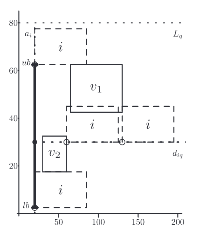
\includegraphics[width=6cm]{multipleassign.png}}
	\caption{Example assigning vessel to multiple locations\TODO{Update Image}}
	\label{fig:multipleassign}
\end{figure}

%%-------------------------------------------------------------------------------
%
\section{Problem Formulation}
\label{sec:problemformulation}
The MILP is formulated with two sets of constraints: queuing constraints and battery dynamics constraints. This section will build off and modify the previous formulation (\eqref{eq:bapobjective} and \eqref{eq:bapconstrs}) and progressively construct the battery dynamic constraints to create the Position Allocation MILP. All notation is defined in Table \ref{tab:variables}.

\subsection{Queuing Constraints}
\noindent
Consider the following set of constraints:

\begin{subequations}
\label{eq:packconstrs}
\begin{align}
    u_i - u_j - p_j - (\sigma_{ij} - 1)T \geq 0                      \label{subeq:time}         \\
    v_i - v_j - s_j - (\delta_{ij} - 1)S \geq 0                      \label{subeq:space}        \\
    \sigma_{ij} + \sigma_{ji} + \delta_{ij} + \delta_{ji} \geq 1     \label{subeq:valid_pos}    \\
    \sigma_{ij} + \sigma_{ji} \leq 1                                 \label{subeq:sigma}        \\
    \delta_{ij} + \delta_{ji} \leq 1                                 \label{subeq:delta}        \\
    p_i + u_i = c_i                                                  \label{subeq:detach}       \\
    a_i \leq u_i \leq (T - p_i)                                      \label{subeq:valid_starts} \\
    c_i \leq \tau_i                                                  \label{subeq:valid_depart} \\
    \sigma_{ij} \in \{0,1\},\;\delta_{ij} \in \{0,1\}                \label{subeq:sdspace}      \\
    v_i \in \{1,2, ... , Q\}                                         \label{subeq:vspace}        \\
\end{align}
\end{subequations}

Constraints \eqref{subeq:time}-\eqref{subeq:valid_starts} are the same as previously described in section \ref{sec:preliminaries}, except charging time \(p\) is now a decision variable. Additionally, starting charge time \(u\) is continuous and charging queue \(v\) discrete as represented in \eqref{subeq:vspace}. Constraint \eqref{subeq:valid_depart} states that the ending charge time \(c\) must be less than or equal to the required departure time from the station \(\tau\).

The constraints \eqref{eq:packconstrs} as stated are flawed. If the objective function given in \eqref{eq:bapobjective} were minimized while being subject to the constraints in \eqref{eq:packconstrs}, \(p\) being defined as a decision variable would naturally cause the solution to converge to 0. This effectively minimizes the objective \(c_i - a_i\), but also would imply no charging should ever be done. To remedy this, battery dynamic constraints will be introduced.

\subsection{Battery Dynamic Constraints}
The battery dynamic constraints are used to drive time spent on the charger \(p\) as well define initial, final, and intermediate bus charges for visit \(i\). Consider the following MILP:

\begin{equation}
\label{eq:objective}
    \sum_{i=1}^N \sum_{q=1}^Q \Big( w_i m_q + g_i \epsilon_q \Big) \\
\end{equation}

Subject to the following constraints:

\begin{subequations}
\label{eq:dynconstrs}
\begin{align}
    \eta_i = \alpha \kappa_{\Gamma_i}                                         \label{subeq:init_charge}  \\
    \eta_i + \sum_{q=1}^Q g_{iq} r_q - \lambda_i = \eta_{\gamma_i}            \label{subeq:next_charge}  \\
    \eta_i + \sum_{q=1}^Q g_{iq} r_q - \lambda_i \geq \nu \kappa_{\Gamma_i}   \label{subeq:min_charge}   \\
    \eta_i + \sum_{q=1}^Q g_{iq} r_q \leq \kappa                              \label{subeq:max_charge}   \\
    \eta_i + \sum_{q=1}^Q g_{iq} r_q - \lambda_i \geq \beta \kappa_{\Gamma_i} \label{subeq:final_charge} \\
    p_i + (1 - w_{iq})M \geq g_{iq}                                           \label{subeq:gpgret}       \\
    p_i \leq g_{iq}                                                           \label{subeq:gples}        \\
    Mw_{iq} \geq g_{iq}                                                       \label{subeq:gwgret}       \\
    0 \leq g_{iq}                                                             \label{subeq:gwles}        \\
    \sum_{q=1}^Q qw_{iq} = v_i                                                \label{subeq:wmax}         \\
    \sum_{q=1}^Q w_{iq} = 1                                                   \label{subeq:wone}         \\
    w_{iq} \in \{0,1\}                                                        \label{subeq:wspace}
\end{align}
\end{subequations}

Constraints \eqref{subeq:init_charge}-\eqref{subeq:final_charge} provide initialization and terminal conditions as well as intermediate constraints to provide continuity in vehicle charges. Constraint \eqref{subeq:init_charge} states the first arrival for each bus is initialized with a charge of \(\alpha \kappa_{\Gamma_i}\). Constraint \eqref{subeq:next_charge} defines that the previous charge \(\eta\) plus the charging done by charger \(q\) minus the discharge amount due to completing route \(\lambda\). Constraints \eqref{subeq:min_charge} is similar to \eqref{subeq:next_charge}, except it states that the charge after being charged by \(q\) and the discharge from route \(\lambda\) must be greater than some percentage of its capacity \(\kappa\). Constraint \eqref{subeq:max_charge} states that the charging done for visit \(i\) cannot be greater than the capacity of the battery \(\kappa\). Constraint \eqref{subeq:final_charge} states that the last visit for each vehicle must have a minimum charge of \(\beta \kappa_{\Gamma_i}\).

The set of constraints \eqref{subeq:gpgret}-\eqref{subeq:gwles} are used to alleviate non-linearity introduced by the bilinear term \(g_{iq} := w_{iq} p_i\). This is accomplished using Big-M notation \cite{Rodriguez2013}. Constraints \eqref{subeq:gpgret} and \eqref{subeq:gples} state that if \(w_{iq} = 1\) then the two equations will take the form of \(p_i \leq g_{eq}\) and \(p_i \geq g_{iq}\) effectively stating \(p_i = g_{iq}\), if \(w_{iq} = 0\) then the two equations will take the form of \(p_i \leq g_{eq}\) and \(p_i \geq g_{iq} - M\) which deactivates the constraint. In a similar fashion, \eqref{subeq:gwgret} and \eqref{subeq:gwles} state if \(w_{iq} = 0\) then the constraints take the form \(0 \geq g_{iq}\) and \(0 \leq g_{iq}\) directly implying \(0 = g_{iq}\). If \(w_{iq} = 1\) then the constraints take the form \(M \leq g_{iq}\) and \(0 \geq g_{iq}\) disabling the constraint. Putting the two sets of constraints together defines the linearized representation of \(w_{iq} p_i\).

The set of constraints \eqref{subeq:wmax}-\eqref{subeq:wone} define the linking constraint between the queuing constraint \(v\) and \(w\) (i.e \(1*w_{iq} + 2*w_{iq} + \cdots = v_i\)) and enforces that only a single \(w\) may be selected per visit, respectively. The last constraint \eqref{subeq:wspace} defines the set of values that \(w\) may be.
% Example
\section{Example}


% There are a few things to note:
% 
% \begin{itemize}
% \item
%   We want to convert this problem to standard LP, for our problem we
%   will mainly be concerned with
% 
%   \begin{itemize}
%   \item
%     Inequality of \(\geq\) form
%   \end{itemize}
% \item
%   We will be formulating the equation in the form \(Ax = b\) and
%   \(Ax \geq b\) where
% 
%   \begin{itemize}
%   \item
%     \(A\) is a \(n \times m\) matrix
%   \item
%     \(x\) is a \(m \times 1\) vector
%   \item
%     \(b\) is a \(n \times 1\) vector
%   \end{itemize}
% \end{itemize}
% 
% 
% \subsection{Position Allocation Problem}
% \subsection{Charging Dynamics}
% 
%%-------------------------------------------------------------------------------

% %%-------------------------------------------------------------------------------
% % Conclusion
% \section{Conclusion}
% 
% \subsubsection{Matrix Deconstruction}\label{matrix-deconstruction}
% 
% The constraint matrix \(A\) will be broken down into two parts:
% \(A_{eq}\) for all the equality constraints and \(A_{ineq}\) for all the
% inequality constraints. Both \(A_{eq}\) and \(A_{ineq}\) formulated with
% two sub-matrices \(A_{pack}\) and \(A_{dynamics}\) to represent the
% portion of the matrix that is utilized for the box packing constraints
% and the battery dynamics constraints, respectively. For example,
% \(A_{eq}\) will be represented in the following manner
% 
% \[
% A_{eq} =
% \begin{bmatrix}
%     A_{\textrm{pack}}     \\
%     A_{\textrm{dynamics}} \\
% \end{bmatrix}_{eq}
% \]
% 
% Where we can define the full equality as:
% 
% \[
% \begin{array}{c}
%     \begin{bmatrix}
%         A_{\textrm{pack}}     \\
%         A_{\textrm{dynamics}} \\
%     \end{bmatrix}_{eq}
%     \begin{bmatrix}
%         x_{\textrm{pack}}     \\
%         x_{\textrm{dynamics}} \\
%     \end{bmatrix}_{eq} =
%     \begin{bmatrix}
%         b_{\textrm{pack}}     \\
%         b_{\textrm{dynamics}} \\
%     \end{bmatrix}_{eq} \\
%     \\
%     A_{eq} x_{eq} = b_{eq} \\
% \end{array}
% \]
% 
% Similarly for the inequality constraints:
% 
% \[
% \begin{bmatrix}
%     A_{\textrm{pack}}     \\
%     A_{\textrm{dynamics}} \\
% \end{bmatrix}_{ineq}
% \begin{bmatrix}
%     x_{\textrm{pack}}     \\
%     x_{\textrm{dynamics}} \\
% \end{bmatrix}_{ineq} \geq
% \begin{bmatrix}
%     b_{\textrm{pack}}     \\
%     b_{\textrm{dynamics}} \\
% \end{bmatrix}_{ineq}
% \]
% 
% Finally, the entire constraint formulation will be written as:
% 
% \begin{subequations}
% \begin{align}
%     \begin{bmatrix}
%         A_{\textrm{pack}}     \\
%         A_{\textrm{dynamics}} \\
%     \end{bmatrix}_{eq}
%     \begin{bmatrix}
%         x_{\textrm{pack}}     \\
%         x_{\textrm{dynamics}} \\
%     \end{bmatrix}_{eq} =
%     \begin{bmatrix}
%         b_{\textrm{pack}}     \\
%         b_{\textrm{dynamics}} \\
%     \end{bmatrix}_{eq} \\
%     \begin{bmatrix}
%         A_{\textrm{pack}}     \\
%         A_{\textrm{dynamics}} \\
%     \end{bmatrix}_{ineq}
%     \begin{bmatrix}
%         x_{\textrm{pack}}     \\
%         x_{\textrm{dynamics}} \\
%     \end{bmatrix}_{ineq} \geq
%     \begin{bmatrix}
%         b_{\textrm{pack}}     \\
%         b_{\textrm{dynamics}} \\
%     \end{bmatrix}_{ineq}
% \end{align}
% \end{subequations}
% 
% \subsection{Formulating $A_{pack}$}
% 
% \subsubsection{Formulating $A_{pack_{eq}}$}
% 
% The components that make up the equality constraints for the box packing
% problem are:
% 
% \begin{itemize}
% \item
%   \(p_i + u_i = c_i\)
% \item
%   \(\sum_{q=1}^Q w_{iq} = 1\)
% \end{itemize}
% 
% Placing them together in \(A_{eq}\) results in:
% 
% \begin{equation}
% \begin{array}{c}
%     A_{eq} =
%     \begin{bmatrix}
%         A_{detach_{N \times 2N}} & \vmathbb{0}_{N \times NQ} \\
%         \vmathbb{0}_{N \times 2N} & A_{w_{N \times NQ}}      \\
%     \end{bmatrix}_{2N \times (2N + NQ)} \\
%     x_{eq} =
%     \begin{bmatrix}
%         p_{i_{N \times 1}} \\
%         u_{i_{N \times 1}} \\
%         w_{iq_{NQ \times 1}} \\
%     \end{bmatrix}_{2N + NQ}
%     b_{eq} =
%     \begin{bmatrix}
%         c_{i_{N \times 1}} \\
%         \vmathbb{1}_{N \times 1} \\
%     \end{bmatrix}_{2N \times 1} \\
%     \\
%     \begin{bmatrix}
%         A_{detach_{N \times 2N}}    & \vmathbb{0}_{N \times NQ} \\
%         \vmathbb{0}_{N \times 2N} & A_{w_{N \times NQ}}          \\
%         \vmathbb{0}_{N \times 2N} & A_{v_{N \times NQ}}          \\
%     \end{bmatrix}
%     \begin{bmatrix}
%         p_{i_{N \times 1}} \\
%         u_{i_{N \times 1}} \\
%         w_{iq_{NQ \times 1}} \\
%     \end{bmatrix}
%     =
%     \begin{bmatrix}
%         c_{i_{N \times 1}} \\
%         \vmathbb{1}_{N \times 1} \\
%         v_{i_{N \times 1}} \\
%     \end{bmatrix}
% \end{array}
% \end{equation}
% 
% Where
% 
% \subsubsection{Formulating $A_{pack_{ineq}}$}
% The components that make up the inequality constraints for the box
% packing problem are
% 
% \begin{itemize}
% \item
%   \(u_j - u_i - p_i - (\sigma_{ij} - 1)T \geq 1\)
% \item
%   \(v_j - v_i - s_i - (\delta_{ij} - 1)S \geq 1\)
% \item
%   \(\sigma_{ij} + \sigma_{ji} + \delta_{ij} + \delta_{ji} \geq 1\)
% \item
%   \(\sigma_{ij} + \sigma_{ji} \leq 1\)
% \item
%   \(\delta_{ij} + \delta_{ji} \leq 1\)
% \item
%   \(a_i \leq c_i \leq (T - p_i)\)
% \item
%   \(c_i \leq \tau_i\)
% \item
%   \(p_i \geq g_{iq}\)
% \item
%   \(p_i \leq g_{iq} - (1 - w_{iq})M\)
% \item
%   \(Mw_{iq} \geq g_{iq}\)
% \item
%   \(0 \leq g_{iq}\)
% \end{itemize}
% 
% \(A_{ineq}\) takes the form of:
% 
% \begin{table*}[!t]
% \begin{equation}
% \setlength{\arraycolsep}{2pt}
% \renewcommand{\arraystretch}{0.8}
% \begin{array}{c}
%     A_{ineq} =
%     \begin{bmatrix}
% 	A_{time_{\Xi \times (2\Xi + 2N)}}    & \vmathbb{0}_{\Xi \times (3\Xi + 4N + 3NQ)} & \cdots                                   & \cdots                     & \cdots                             & \cdots                           & \cdots                     & \cdots                & \cdots                    \\
% 	\vmathbb{0}_{\Xi \times (2\Xi + 2N)} & A_{queue_{\Xi \times (2\Xi + 2N)}}         & \vmathbb{0}_{\Xi \times (\Xi + 2N)}      & \cdots                     & \cdots                             & \cdots                           & \cdots                     & \cdots                & \cdots                    \\
% 	\vmathbb{0}_{N \times 2N}            & A_{\sigma_{N \times \Xi}}                  & \vmathbb{0}_{N \times (2N + 3NQ)}        & A_{\delta_{N \times \Xi}}  & \vmathbb{0}_{N \times (2\Xi + 2N)} & \cdots                           & \cdots                     & \cdots                & \cdots                    \\
% 	\vmathbb{0}_{N \times 2N}            & -A_{\sigma_{N \times \Xi}}                 & \vmathbb{0}_{N \times (3\Xi + 4N + 3NQ)} & \cdots                     & \cdots                             & \cdots                           & \cdots                     & \cdots                & \cdots                    \\
% 	\vmathbb{0}_{N \times (2\Xi + 2N)}   & \vmathbb{0}_{N \times (2N)}                & \cdots                                   & -A_{\delta_{N \times \Xi}} & \vmathbb{0}_{N \times (2N + 3NQ)}  & \cdots                           & \cdots                     & \cdots                & \cdots                    \\
% 	\vmathbb{0}_{N \times (4\Xi + 4N)}   & \cdots                                     & \cdots                                   & \cdots                     & -A_{a_{N \times N}}                & \vmathbb{0}_{N \times (N + 3NQ)} & \cdots                     & \cdots                & \cdots                    \\
% 	\vmathbb{0}_{N \times (4\Xi + 5N)}   & \cdots                                     & \cdots                                   & \cdots                     & \cdots                             & -A_{c_{N \times N}}              & \vmathbb{0}_{N \times 3NQ} & \cdots                & \cdots                    \\
% 	\vmathbb{0}_{N \times (4\Xi + 5N)}   & \cdots                                     & \cdots                                   & \cdots                     & \cdots                             & -A_{c_{N \times N}}              & \vmathbb{0}_{N \times 3NQ} & \cdots                & \cdots                    \\
% 	\vmathbb{0}_{4N \times (4\Xi + 6N)}  & \cdots                                     & \cdots                                   & \cdots                     & \cdots                             & \cdots                           & A_{gg_{4N \times NQ}}      & A_{gw_{4N \times NQ}} & \vmathbb{1}_{4N \times NQ} \\
%     \end{bmatrix}_{(2\Xi + 10N) \times (4\Xi + 6N + 3NQ)}                                                                                                                                                                                                                                                                       \\
% 	\\
%     x_{ineq} =
%     \begin{bmatrix}
% 	u_{i_{N \times 1}} \\ p_{i_{N \times 1}} \\ \sigma_{ij_{\Xi \times 1}} \\ \vmathbb{1}_{\Xi \times 1} \\ v_{i_{N \times 1}} \\ s_{i_{N \times 1}} \\ \delta_{ij_{\Xi \times 1}} \\ \vmathbb{1}_{\Xi \times 1} \\ a_{i_{N \times 1}} \\ c_{i_{N \times 1}} \\ q_{iq_{NQ \times1}} \\w_{iq_{NQ \times 1}} \\ \vmathbb{1}_{NQ \times 1} \\
%     \end{bmatrix}_{(4\Xi + 6N + 3NQ) \times 1}
%     b_{ineq} =
%     \begin{bmatrix}
% 	\vmathbb{1}_{\Xi \times 1} \\ \vmathbb{1}_{\Xi \times 1} \\ \vmathbb{1}_{N \times 1} \\ -\vmathbb{1}_{N \times 1} \\ -\vmathbb{1}_{N \times 1} \\ -c_{i_{N \times N}} \\ -(T-p_i)_{N \times N} \\ -\tau_{i_{N \times N}} \\ -p_{i_{N \times 1}} \\ p_{i_{N \times 1}} \\ \vmathbb{0}_{2N \times 1}
%     \end{bmatrix}_{(5\Xi + 7N) \times 1}
% \end{array}
% \end{equation}\\
% \end{table*}
% 
% \subsection{Formulating $A_{dynamics}$}
% 
% \subsubsection{Formulating $A_{dynamics_{eq}}$}
% The components that make up the equality constraint for the dynamics problem are
% 
% \begin{itemize}
%     \item
%     $\eta_{\gamma_i} = \eta_i + g_{iq} r_q - \lambda_i$
% \end{itemize}
% 
% $A_{dynamics}$ takes the form of:
% 
% \begin{equation}
% \begin{array}{c}
% 	A_{eq} =
% 	\begin{bmatrix}
% 		A_{\textrm{init charge}_{N \times N}}       & \vmathbb{0}_{N \times (N+NQ)} \\
% 		A_{\textrm{next charge}_{N \times 2N + NQ}} & \cdots                       \\
% 	\end{bmatrix}_{2N \times (2N + NQ)} \\
% 	x_{eq} =
% 	\begin{bmatrix}
% 		\eta_{\i_{N \times 1}}   \\
% 		g_{iq_{NQ \times 1}}     \\
% 		\lambda_{i_{N \times 1}} \\
% 	\end{bmatrix}_{(2N + NQ) \times 1}
% 	b_{eq} =
% 	\begin{bmatrix}
% 		\eta_{i_{N \times 1}} \\
% 		\eta_{\gamma_{i}\; N \times 1} \\
% 	\end{bmatrix}_{2N \times 1}
% \end{array}
% \end{equation}
% 
% \(A_{dyanmics_{ineq}}\) takes the form of:
% 
% \begin{equation}
% \begin{array}{c}
%     A_{ineq} =
%     \begin{bmatrix}
% 	-A_{\textrm{max charge}_{N \times (N+NQ)}} & \vmathbb{0}_{N \times N}        \\
% 	A_{\textrm{min charge}_{N \times (2N+NQ)}} & \cdots                         \\
% 	A_{\textrm{last charge}_{N \times N}}      & \vmathbb{0}_{N \times (N + NQ)} \\
%     \end{bmatrix}_{3N \times (2N + NQ)} \\
%     x_{ineq} =
%     \begin{bmatrix}
% 	\eta_{i_{N \times 1}} \\
% 	g_{iq_{NQ \times 1}} \\
%     \end{bmatrix}_{(2N + NQ) \times 1}
%     b_{ineq} =
%     \begin{bmatrix}
% 	-\vmathbb{1}_{N + NQ \times 1} \\
% 	\vmathbb{0}_{2N + NQ \times 1} \\
% 	H_{final}*\vmathbb{1}_{A \times 1} \\
%     \end{bmatrix}_{3N \times 1}
% \end{array}
% \end{equation}
% 
% \subsection{Putting it back together}\label{putting-it-back-together}
% 
% \begin{equation*}
% \begin{array}{c}
%     \begin{bmatrix}
% 	A_{\textrm{pack}}     \\
% 	A_{\textrm{dynamics}} \\
%     \end{bmatrix}_{eq}
%     \begin{bmatrix}
% 	x_{\textrm{pack}}     \\
% 	x_{\textrm{dynamics}} \\
%     \end{bmatrix}_{eq} =
%     \begin{bmatrix}
% 	b_{\textrm{pack}}     \\
% 	b_{\textrm{dynamics}} \\
%     \end{bmatrix}_{eq} \\
%     \begin{bmatrix}
% 	A_{\textrm{pack}}     \\
% 	A_{\textrm{dynamics}} \\
%     \end{bmatrix}_{ineq}
%     \begin{bmatrix}
% 	x_{\textrm{pack}}     \\
% 	x_{\textrm{dynamics}} \\
%     \end{bmatrix}_{ineq} \geq
%     \begin{bmatrix}
% 	b_{\textrm{pack}}     \\
% 	b_{\textrm{dynamics}} \\
%     \end{bmatrix}_{ineq}
% \end{array}
% \end{equation*}
% 
% May also be represented as
% 
% \scriptsize
% 
% \begin{equation}
% \begin{array}{c}
% A_{eq} =
% \begin{bmatrix}
%     \begin{Bmatrix}
% 	A_{detach_{N \times 2N}}    & \vmathbb{0}_{N \times NQ} \\
% 	\vmathbb{0}_{N \times 2N} & A_{w_{N \times NQ}}          \\
% 	\vmathbb{0}_{N \times 2N} & A_{v_{N \times NQ}}          \\
%     \end{Bmatrix}_{3N \times (2N + NQ)}
%     \begin{Bmatrix}
% 	\vmathbb{0}
%     \end{Bmatrix}_{3N \times (2N + NQ)} \\
%     \begin{Bmatrix}
% 	\vmathbb{0}_{}
%     \end{Bmatrix}_{NA \times (2N + NQ)}
%     \begin{Bmatrix}
% 	A_{\textrm{next charge}_{N \times 2N + NQ}}
%     \end{Bmatrix}_{NA \times (2N + NQ + A)} \\
% \end{bmatrix}_{(3N + NA) \times (4N + NQ + A)} \\
% x_{eq} =
% \begin{bmatrix}
%     \begin{Bmatrix}
% 	p_{i_{N \times 1}} \\
% 	u_{i_{N \times 1}} \\
% 	w_{iq_{NQ \times 1}} \\
%     \end{Bmatrix}_{2N + NQ} \\
%     \begin{Bmatrix}
% 	\eta_{\Gamma_{i\; N \times 1}} \\
% 	g_{iq_{NQ \times 1}}           \\
% 	\lambda_{i_{N \times 1}}       \\
%     \end{Bmatrix}_{(2N + NQ + A) \times 1}
% \end{bmatrix}_{(4N + 2NQ + A) \times 1}
% b_{eq} =
% \begin{bmatrix}
%     \begin{Bmatrix}
% 	c_{i_{N \times 1}} \\
% 	\vmathbb{1}_{N \times 1} \\
% 	v_{i_{N \times 1}} \\
%     \end{Bmatrix}_{3N \times 1} \\
%     \begin{Bmatrix}
% 	\eta_{\gamma_{i}\; N \times 1} \\
%     \end{Bmatrix}_{N \times 1}
% \end{bmatrix}_{4N \times 1} \\
% \begin{bmatrix}
%     \begin{Bmatrix}
% 	A_{detach_{N \times 2N}}    & \vmathbb{0}_{N \times NQ} \\
% 	\vmathbb{0}_{N \times 2N} & A_{w_{N \times NQ}}          \\
% 	\vmathbb{0}_{N \times 2N} & A_{v_{N \times NQ}}          \\
%     \end{Bmatrix}_{3N \times (2N + NQ)}
%     \begin{Bmatrix}
% 	\vmathbb{0}
%     \end{Bmatrix}_{3N \times (2N + NQ)} \\
%     \begin{Bmatrix}
% 	\vmathbb{0}_{}
%     \end{Bmatrix}_{NA \times (2N + NQ)}
%     \begin{Bmatrix}
% 	A_{\textrm{next charge}_{N \times 2N + NQ}}
%     \end{Bmatrix}_{NA \times (2N + NQ + A)} \\
% \end{bmatrix}
% \begin{bmatrix}
%     \begin{Bmatrix}
% 	p_{i_{N \times 1}} \\
% 	u_{i_{N \times 1}} \\
% 	w_{iq_{NQ \times 1}} \\
%     \end{Bmatrix}_{2N + NQ} \\
%     \begin{Bmatrix}
% 	\eta_{\Gamma_{i\; N \times 1}} \\
% 	g_{iq_{NQ \times 1}}           \\
% 	\lambda_{i_{N \times 1}}       \\
%     \end{Bmatrix}_{(2N + NQ + A) \times 1}
% \end{bmatrix} \\
% =
% \begin{bmatrix}
%     \begin{Bmatrix}
% 	c_{i_{N \times 1}} \\
% 	\vmathbb{1}_{N \times 1} \\
% 	v_{i_{N \times 1}} \\
%     \end{Bmatrix}_{3N \times 1} \\
%     \begin{Bmatrix}
% 	\eta_{\gamma_{i}\; N \times 1} \\
%     \end{Bmatrix}
% \end{bmatrix}_{4N \times 1}
% \end{array}
% \end{equation}

%%================================================================================
% Bibliography
\bibliographystyle{IEEEtran}
\bibliography{main}

%%%%%%%%%%%%%%%%%%%%%%%%%%%%%%%%%%%%%%%%%%%%%%%%%%%%%%%%%%%%%%%%%%%%%%%%%%%%%%%%%
\end{document}
